\chapter{Einführung und Ziele}

\section{Aufgabenstellung}

Es soll ein verteiltes Steuerungssystem gemäß den Prinzipien verteilter Systeme nach Tanenbaum \& van Steen entworfen und implementiert werden. Über ein ITS-Board (bspw. STM32F4) soll ein autonomer Roboter innerhalb eines kontrollierten Areals (z.B. BT7 R7.65 – als realer Testbereich) sicher und effizient gesteuert werden. Die verteilte Architektur soll dabei explizit gewährleisten, dass durch Fehlverhalten der Software oder Architektur keine Gefahr für anwesende entstehen kann.


\subsection*{Use Case Diagramm} % TODO make this the label/caption

\begin{figure}[h]
	\centering
	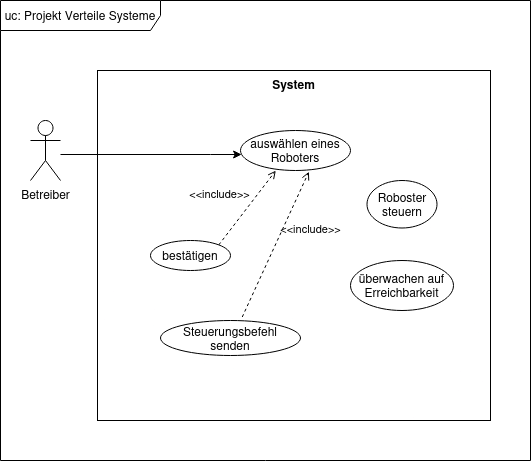
\includegraphics[scale=.5]{diagrams/use_case.png}
	\caption{Funktionales Use Case Diagramm der Aufgabenstellung}
	\label{fig:meine-grafik}
\end{figure}


\section{Qualitätsziele}
% Aus VS Skript Kapitel 2.4 Seite 23
% TODO zu jeden Punkt eine Definition oder entfernen
% TODO messbar definieren

Das verteilte Steuerungssystem soll eine Reihe von nicht-funktionalen Anforderungen erfüllen, um einen sicheren, wartbaren und erweiterbaren Betrieb im Einsatzumfeld zu gewährleisten. 

\subsection{Ziele für Software Engineering}
\begin{table}[h!]
    \centering
    \begin{tabular}{p{4cm}|p{10cm}}
        \hline
        \textbf{Ziel} & \textbf{Beschreibung} \\
        \hline
        Funktionalität & 
        %Der Roboter muss Steuerbefehle korrekt umsetzen, auf Umgebungsdaten reagieren und vordefinierte Aufgaben zuverlässig erfüllen.
        \\
        Zuverlässigkeit & 
        %Teilausfälle dürfen den Gesamtsystembetrieb nicht gefährden. Fehlererkennung und -toleranz müssen integriert sein. 
        \\
        Skalierbarkeit & 
        %Zusätzliche Roboter oder Komponenten sollen ohne Änderungen an der bestehenden Architektur integrierbar sein. 
        \\
        Leistung & 
        %Reaktionszeiten auf Steuerbefehle und Ereignisse müssen innerhalb definierter Zeitgrenzen liegen. 
        \\
        Sicherheit (Safety) & 
        %Das System darf unter keinen Umständen eine Gefährdung für Kinder darstellen. Bei Fehlern muss sofort ein sicherer Zustand erreicht werden (z.B. Notstopp). 
        \\
        Wartbarkeit & 
        %Der Code muss modular, gut dokumentiert und testbar sein. Fehlerdiagnose und Protokollierung sollen integriert sein. 
        \\
        Portabilität & %Die Software soll ohne großen Aufwand auf vergleichbaren Embedded-Systemen lauffähig sein. 
        \\
        Benutzerfreundlichkeit & %Konfiguration und Überwachung müssen intuitiv bedienbar und gut visualisiert sein. 
        \\
        Anpassbarkeit & 
        %Neue Funktionen, Sensoren oder Regeln sollen ohne tiefgreifende Änderungen am System integrierbar sein. 
        \\
        Kompatibilität & 
        %Das System soll mit bestehenden Standards und Protokollen kommunizieren können. 
        \\
        \hline
    \end{tabular}
    \caption{Qualitätsziele der Software Engineering}
    \label{tab:qualitaetsziele}
\end{table}

\clearpage
\subsection{Ziele der Verteilte Systeme}
    \begin{table}[h!]
        \centering
        \begin{tabular}{p{4cm}|p{10cm}}
            \hline
            \textbf{Ziel} & \textbf{Beschreibung} \\
            \hline
            Ressourcenteilung  & ...\\
            Offenheit & ...\\
            Skalierbarkeit & ...\\
            Verteilung Transparenz & ...\\
            \hline
        \end{tabular}
        \caption{Qualitätsziele der Verteilten Systeme}
        \label{tab:qualitaetsziele}
    \end{table}
    
\subsubsection{Skalierbarkeit}
    \begin{table}[h!]
            \centering
            \begin{tabular}{p{4cm}|p{10cm}}
                \hline
                \textbf{Ziel} & \textbf{Beschreibung} \\
                \hline
                Vertikale Skalierung   & ...\\
                Horizontale Skalierung & ...\\
                Räumliche Skalierbarkeit &  1\\
                Funktionale Skalierbarkeit & ...\\
                Administrative-Skalierbarkeit & 1 \\
                \hline
            \end{tabular}
            \caption{Skalierbarkeiten}
            \label{tab:qualitaetsziele}
        \end{table}
    
\newpage
\subsubsection{Verteilungs-Transparenzen}
    \begin{table}[h!]
            \centering
            \begin{tabular}{p{4cm}|p{10cm}}
                \hline
                \textbf{Ziel} & \textbf{Beschreibung} \\
                \hline
                Zugriffstransparenz   & ...\\
                Lokalitäts-Transparenz  & ...\\
                Migrationstransparenz & ...\\
                Replikationstransparenz &...\\
                Fehlertransparenz &... \\
                Ortstransparenz & .. \\
                Skalierbarkeits-Transparenz &...\\
                %Concurrency
                %Relocation
                \hline
            \end{tabular}
            \caption{Verteilungs-Transparenzen}
            \label{tab:qualitaetsziele}
        \end{table}
        



\clearpage
\section{Stakeholder}
Die folgenden Gruppen sind direkt oder indirekt vom System betroffen:

\begin{itemize}
    \item \textbf{Endnutzer:} Personen, die mit dem Roboter interagieren (z.B. Lehrpersonal, Kinder im Testbereich)
    \item \textbf{Entwicklerteam:} Zuständig für Entwurf, Umsetzung, Tests und Wartung des Systems
    \item \textbf{Betreiber:} Verantwortlich für die Überwachung und den sicheren Betrieb des Systems im realen Umfeld
    \item \textbf{Professor:} Person, die für die Bewertung des Systems verantwortlich ist und vorgabe der Rahmenbedingungen.

\end{itemize}
